\documentclass{sbc2023}%

\usepackage{graphicx}
%\usepackage[utf8]{inputenc}
\usepackage[misc,geometry]{ifsym} 
\usepackage{float}
\usepackage{fontspec}
\usepackage{fontawesome}
\usepackage{academicons}
\usepackage{color}
\usepackage{hyperref} 
\usepackage{aas_macros}
\usepackage[bottom]{footmisc}
\usepackage{supertabular}
\usepackage{afterpage}
\usepackage{url}
\usepackage{pifont}
\usepackage{multicol}
\usepackage{multirow}

\setcitestyle{square}

\definecolor{orcidlogo}{rgb}{0.37,0.48,0.13}
\definecolor{unilogo}{rgb}{0.16, 0.26, 0.58}
\definecolor{maillogo}{rgb}{0.58, 0.16, 0.26}
\definecolor{darkblue}{rgb}{0.0,0.0,0.0}
\hypersetup{colorlinks,breaklinks,
            linkcolor=darkblue,urlcolor=darkblue,
            anchorcolor=darkblue,citecolor=darkblue}
%\hypersetup{colorlinks,citecolor=blue,linkcolor=blue,urlcolor=blue}

%%%%%%% IMPORTANT: We disable hyperlinks by default with this line, to avoid the error "\pdfendlink ended up in different nesting level" while writing.
%\hypersetup{draft}

\jid{JBCS}
\jtitle{Journal of the Brazilian Computer Society, 202X, XX:1, }
\doi{10.5753/jbcs.202X.XXXXXX}
\copyrightstatement{This work is licensed under a Creative Commons Attribution 4.0 International License}
\jyear{202X}

\title{Distância de Edição em Estruturas Hierárquicas: Um Estudo entre Algoritmo Exato e Heurística Aproximada}

%THE ORCID IS MANDATORY FOR EACH AUTHOR IN JBCS
\author[Gualtieri et al. 2025] {

    \affil{\textbf{Lucas Gualtieri}
    ~[~\textbf{PUC Minas} |
    {~\textbf{\textit{lgualtieri@sga.pucminas.br}}}~]}

    \affil{\textbf{Gabriel Quaresma}
    ~[~\textbf{PUC Minas} |
    {~\textbf{\textit{gabrie.oliveira.1462924@sga.pucminas.br}}}~]}

    \affil{\textbf{Luca Gonzaga}
    ~[~\textbf{PUC Minas} |
    {~\textbf{\textit{lucalourenco@gmail.com}}}~]}

    \affil{\textbf{Pedro Alves}
    ~[~\textbf{PUC Minas} |
    {~\textbf{\textit{Pedro.alves.1446100@sga.pucminas.br}}}~]}

}

\begin{document}

\begin{frontmatter}
\maketitle

\begin{mail}
Pontifical Catholic University of Minas Gerais, R. Dom José Gaspar, 500 - Coração Eucarístico, Belo Horizonte - MG, 30535-901. 
\end{mail}

\begin{abstract}
Tree Edit Distance (TED) is a well-established metric for measuring structural similarity between trees, with applications ranging from computational biology to image analysis. This paper presents a comparative study between two approaches for calculating TED: the exact algorithm proposed by Zhang and Shasha (1989), and a heuristic method based on tree serialization followed by Levenshtein distance calculation. The study includes the implementation of both algorithms and an experimental evaluation using synthetic datasets with varying tree topologies and sizes. Results show that while the Zhang and Shasha algorithm offers precise distance computation at higher computational cost, the heuristic approach provides significant runtime improvements with acceptable approximation for large trees. The trade-offs between accuracy and performance are discussed, offering insights into the suitability of each method for different application contexts.
\end{abstract}


\begin{keywords}
Tree Edit Distance, Zhang and Shasha Algorithm, Levenshtein Distance, Approximation Heuristics, Tree Comparison, Computational Efficiency.
\end{keywords}


%\begin{license}
%Published under the Creative Commons Attribution 4.0 International Public License (CC BY 4.0)
%\end{license}

\end{frontmatter}

\section{Introdução}
 
A distância de edição entre árvores (Tree Edit Distance, TED) é uma medida clássica de similaridade estrutural entre duas árvores. Ela é definida como o número mínimo de operações (substituição, inserção ou remoção de vértices) necessárias para transformar uma árvore T1 em outra árvore T2. Essa métrica tem aplicações importantes em diversas áreas, como comparação de estruturas secundárias de RNA, árvores filogenéticas e análise hierárquica de imagens.

Neste trabalho, implementamos o algoritmo proposto por \cite{doi:10.1137/0218082}, que é um dos algoritmos mais conhecidos para cálculo exato da TED em árvores ordenadas, e o comparamos com um segundo método baseado em heurística via serialização e aplicação da distância de Levenshtein.
\section{Objetivo}

O objetivo deste trabalho é:

\begin{itemize}
\item Implementar o algoritmo exato de \cite{doi:10.1137/0218082} para distância de edição entre árvores.
\item Implementar um segundo algoritmo de comparação de árvores baseado em heurística.
\item Comparar os dois métodos em relação ao tempo de execução e a diferença absoluta das TEDs (Tree Edit Distance) encontradas, conforme o tamanho das árvores aumenta.
\end{itemize}

\section{Metodologia}

\subsection{Algoritmo de Zhang \& Shasha (1989)}

Este algoritmo utiliza programação dinâmica para calcular a distância de edição entre árvores ordenadas. Ele é baseado na decomposição das árvores em florestas e no reuso de resultados de subproblemas.

\begin{itemize}
\item Complexidade: \(O(n^3)\) no pior caso.
\item Entrada: duas árvores ordenadas com rótulos.
\item Saída: distância de edição entre as duas árvores.
\end{itemize}

\subsection{Segundo Método: Serialização + Levenshtein}

Neste método alternativo, transformamos cada árvore em uma string por meio de uma travessia em pré-ordem e comparamos as duas strings utilizando a distância de Levenshtein.

\begin{itemize}
\item Complexidade: \(O(n^2)\) para Levenshtein + custo de serialização.
\item Vantagem: simples e eficiente para grandes instâncias.
\item Desvantagem: perde informação estrutural da árvore.
\end{itemize}

\subsection{Geração de Dados}

Utilizamos um gerador de árvores com diferentes topologias:

\begin{itemize}
\item Árvores binárias completas
\item Árvores lineares
\item Árvores estrela
\item Árvores aleatórias
\item Árvores rasas (de baixa altura)
\end{itemize}

Os tamanhos variaram de \(2^3\) até \(2^{10}\) nós.

\section{Resultados Experimentais}

\subsection{Métricas Avaliadas}

\begin{itemize}
\item Tempo de execução (em segundos)
\item Distância de edição (valor absoluto)
\end{itemize}

\subsection{Metodologia de Execução}

\begin{itemize}
\item As árvores foram carregadas a partir de arquivos binários.
\item Os algoritmos foram executados para todos os pares de árvores.
\item Cada execução foi repetida várias vezes para cálculo da média.
\item Os resultados foram salvos em arquivos CSV para análise posterior.
\end{itemize}

\subsection{Resultados Obtidos}

\begin{figure}[htbp]
    \centering
    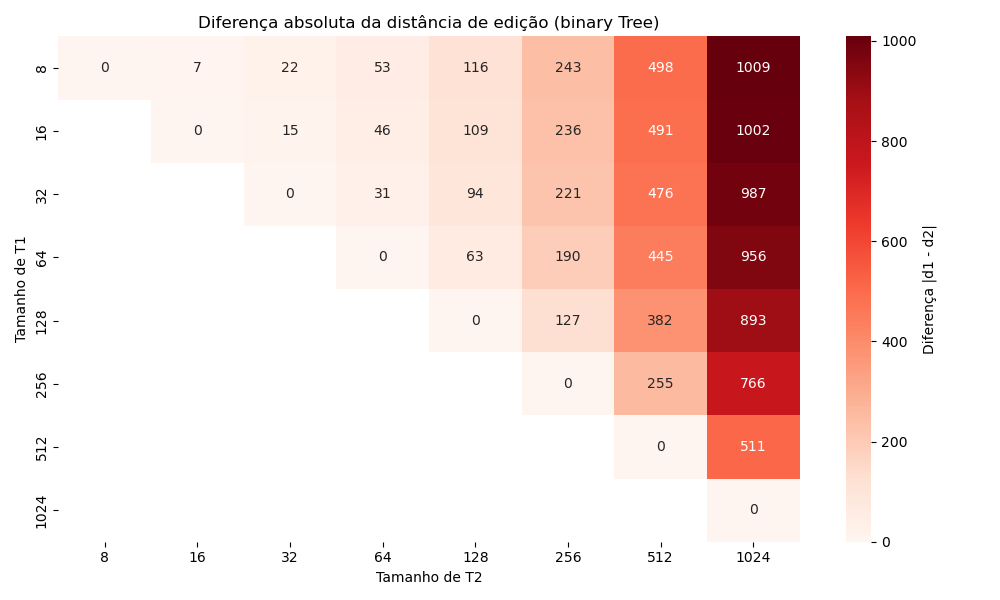
\includegraphics[width=0.5\textwidth]{images/heatmap_diff_edit_distance_binary_tree.png}
    \caption{ Diferença absoluta da distância de edição em árvores binárias. }
    \label{fig:exemplo}
\end{figure}

\begin{figure}[htbp]
    \centering
    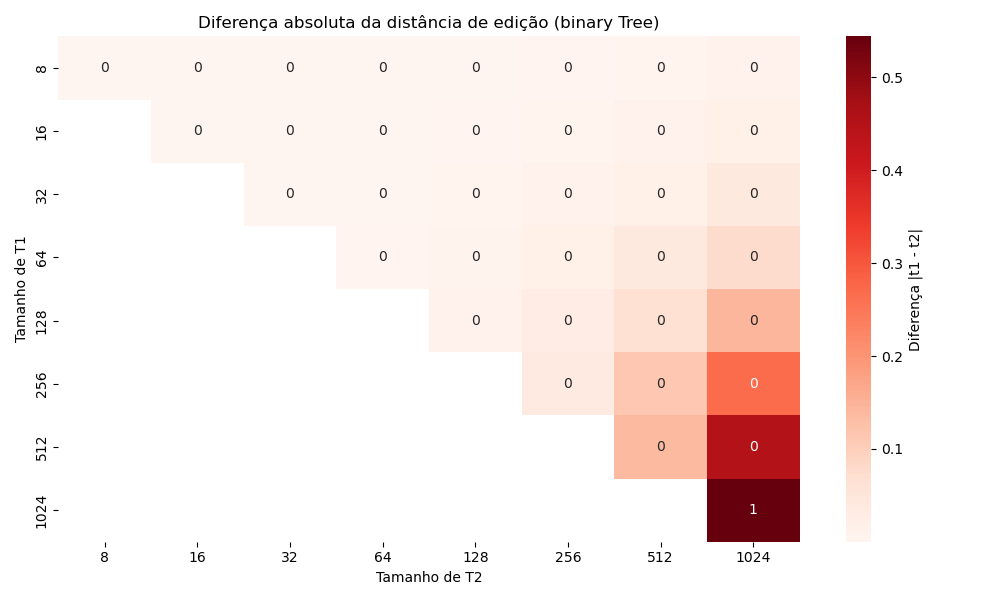
\includegraphics[width=0.5\textwidth]{images/heatmap_diff_time_taken_binary_tree.png}
    \caption{ Diferença absoluta do tempo de execução dos algoritmos em árvores binárias. }
    \label{fig:exemplo}
\end{figure}

% -------------------------------------------------------------------------------------------------

\begin{figure}[htbp]
    \centering
    % \includegraphics[width=0.5\textwidth]{images/heatmap_diff_edit_distance_linear_tree.png}
    \caption{ Diferença absoluta da distância de edição em árvores lineares (Grafo de Linha). }
    \label{fig:exemplo}
\end{figure}

\begin{figure}[htbp]
    \centering
    % \includegraphics[width=0.5\textwidth]{images/heatmap_diff_time_taken_linear_tree.png}
    \caption{ Diferença absoluta do tempo de execução dos algoritmos em árvores lineares (Grafo de Linha). }
    \label{fig:exemplo}
\end{figure}

% -------------------------------------------------------------------------------------------------

\begin{figure}[htbp]
    \centering
    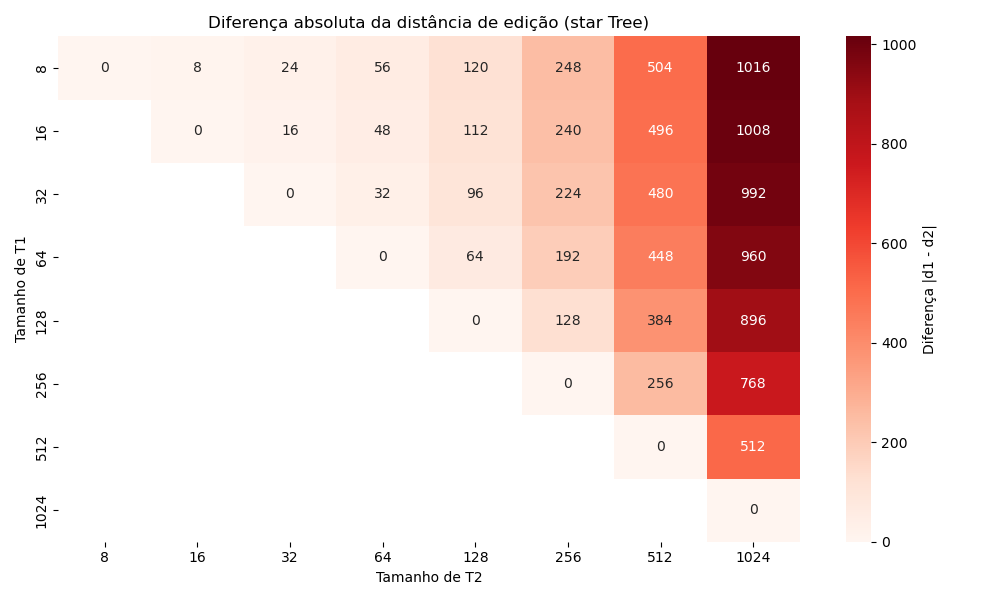
\includegraphics[width=0.5\textwidth]{images/heatmap_diff_edit_distance_star_tree.png}
    \caption{ Diferença absoluta da distância de edição em árvores estrela. }
    \label{fig:exemplo}
\end{figure}

\begin{figure}[htbp]
    \centering
    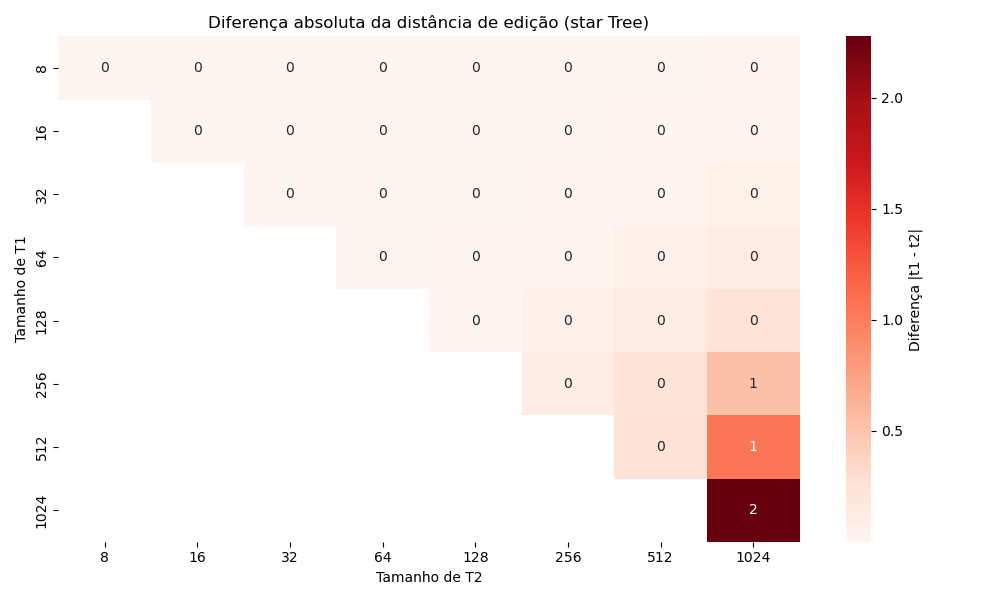
\includegraphics[width=0.5\textwidth]{images/heatmap_diff_time_taken_star_tree.png}
    \caption{ Diferença absoluta do tempo de execução dos algoritmos em árvores estrela. }
    \label{fig:exemplo}
\end{figure}

% -------------------------------------------------------------------------------------------------

\begin{figure}[htbp]
    \centering
    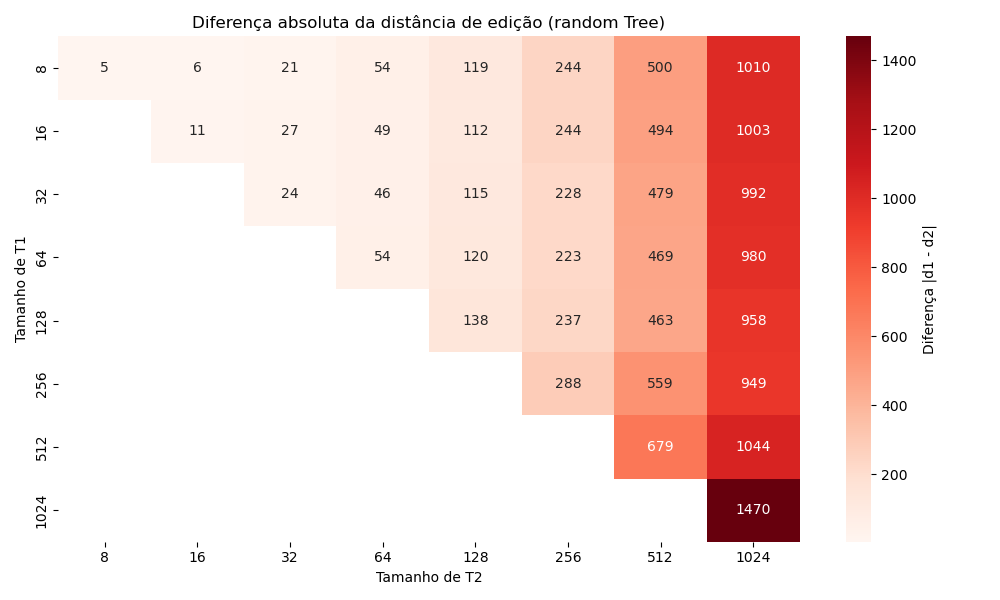
\includegraphics[width=0.5\textwidth]{images/heatmap_diff_edit_distance_random_tree.png}
    \caption{ Diferença absoluta da distância de edição em árvores aleatórias. }
    \label{fig:exemplo}
\end{figure}

\begin{figure}[htbp]
    \centering
    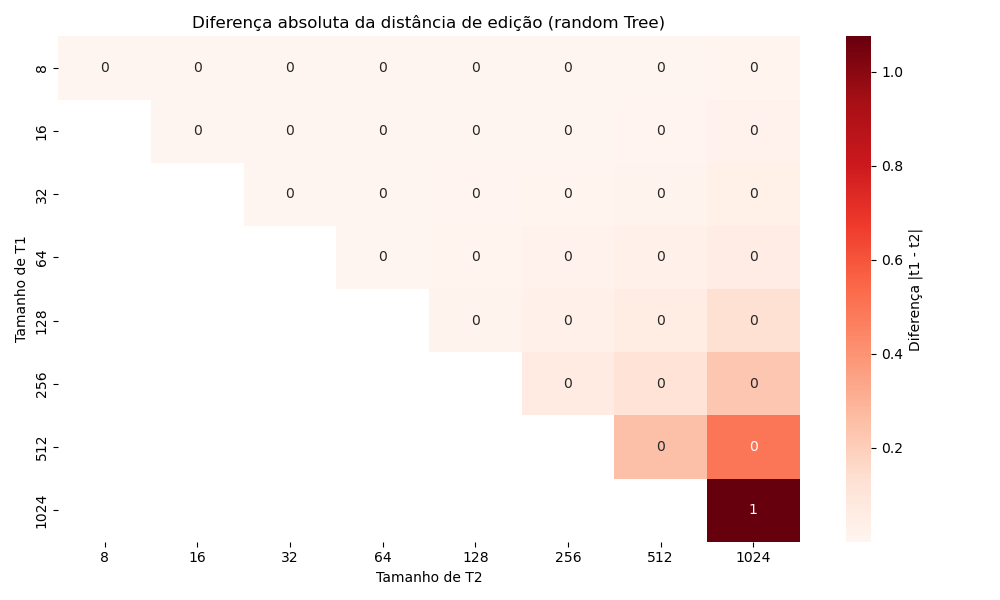
\includegraphics[width=0.5\textwidth]{images/heatmap_diff_time_taken_random_tree.png}
    \caption{ Diferença absoluta do tempo de execução dos algoritmos em árvores aleatórias. }
    \label{fig:exemplo}
\end{figure}

% -------------------------------------------------------------------------------------------------

\begin{figure}[htbp]
    \centering
    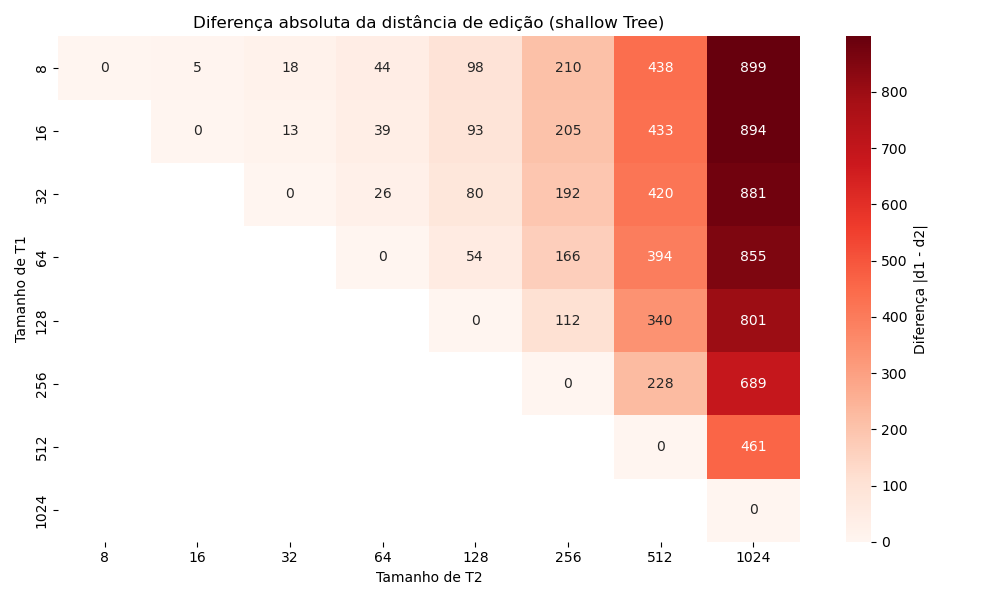
\includegraphics[width=0.5\textwidth]{images/heatmap_diff_edit_distance_shallow_tree.png}
    \caption{ Diferença absoluta da distância de edição em árvores aleatórias de baixa altura. }
    \label{fig:exemplo}
\end{figure}

\begin{figure}[htbp]
    \centering
    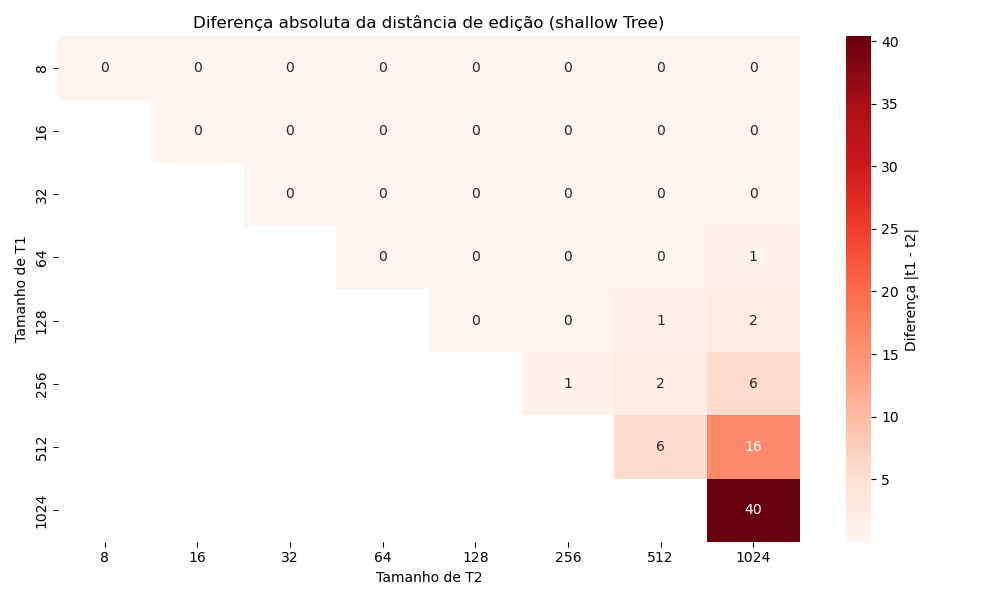
\includegraphics[width=0.5\textwidth]{images/heatmap_diff_time_taken_shallow_tree.png}
    \caption{ Diferença absoluta do tempo de execução dos algoritmos em árvores aleatórias de baixa altura. }
    \label{fig:exemplo}
\end{figure}

Resumo dos resultados:

\begin{itemize}
\item O algoritmo de \cite{doi:10.1137/0218082} apresentou crescimento cúbico em tempo.
\item O método heurístico foi mais rápido, mas muito menos preciso.
\end{itemize}

\section{Discussão}

Os resultados confirmam as expectativas teóricas: o algoritmo de \cite{doi:10.1137/0218082} é ótimo, portanto sempre encontra a menor TED, mas seu custo pode se tornar impraticável para certas aplicações. A abordagem heurística é útil quando a eficiência é mais importante do que a otimalidade. Os heatmaps revelam que o algoritmo heurístico, apesar de seu excelente desempenho em tempo, produz estimativas de distância significativamente inferiores àquelas fornecidas pelo algoritmo de Zhang \& Shasha, especialmente em árvores de grande porte e topologias mais complexas, como árvores aleatórias. A discrepância ultrapassa 1000 unidades em diversos casos, o que compromete a aplicabilidade do método em contextos sensíveis à exatidão da métrica. Em contrapartida, a eficiência temporal do método heurístico o torna útil em aplicações com restrições de tempo ou com tolerância a aproximações.

\section{Conclusão}

Este trabalho demonstrou, de forma experimental, as diferenças entre dois métodos para calcular distância de edição entre árvores. O algoritmo de \cite{doi:10.1137/0218082} continua sendo uma referência para comparação exata, enquanto métodos heurísticos podem ser utilizados em cenários que exigem desempenho.

% \section*{Referência}

% % Zhang, Kaizhong and Dennis Shasha (1989). “Simple Fast Algorithms for the Editing Distance between Trees and Related Problems”. In: \textit{SIAM Journal on Computing} 18.6, pp. 1245–1262. doi: \href{https://doi.org/10.1137/0218082}{10.1137/0218082}

\section*{Contributions}

As contribuições de cada membros foram como mostrado à seguir:\\
\textbf{Lucas Gualtieri:} Implementou o algoritmo de Zhang \& Sasha e estruturou os experimentos.\\
\textbf{Gabriel Quaresma:} Implementou o Algoritmo de Serialização + Levenshtein e estruturou os experimentos. \\
\textbf{Luca Gonzaga:} Estruturou os experimentos e documentou o experimento. \\
\textbf{Pedro Alves:} Implementou estruturas de dados auxiliares e documentou o experimento. \\


\bibliographystyle{apalike-sol}
\bibliography{refs}

\end{document}